%% freie_software.tex
%% $Id: freie_software.tex 61 2012-05-03 13:58:03Z bless $

\chapter{Gliederungsentwurf und Ablaufplan}
\label{ch:FreieSoftware}
%% ==============================

In diesem Kapitel wird die vorläufige inhaltliche Gliederung der Bachelor-Thesis behandelt. 
Diese zeigt den aktuellen IST-Stand und kann sich zur endgültigen Finalversion noch geringfügig ändern.
Weiter wird der Zeit- und Ablaufplan präsentiert, welcher lediglich zur anschaulichen Darstellung der einzelnen Vorgehensschritte dient.
  
%% ==============================
\section{Gliederungsentwurf}
%% ==============================
\label{ch:FreieSoftware:sec:Gliederung}

Die nachfolgende Gliederung zeigt den derzeitigen Stand des Inhaltsverzeichnisses der Bachelor-Thesis. Dieses kann sich im Laufe der Ausarbeitung noch geringfügig ändern und so in der finalen Version leicht abweichen.

\begin{center}
\begin{description}
\item[Inhaltsverzeichnis]~\par
   \begin{enumerate}
      \item Einleitung
      \begin{enumerate}
         \item Ausgangssituation
         \item Problemstellung
         \item Zielsetzung
         \item Vorgehensweise und Aufbau der Arbeit
      \end{enumerate}
      \item IT - The State of Art
      \begin{enumerate}
      	\item An- und Herausforderungen an IT-Organisationen
	\item IT Geschäftsprozesse
	\begin{enumerate}
		\item Definition
		\item Bedeutung und Ausrichtung
	\end{enumerate}
	\item IT Service Management
	\item Zusammenfassung
      \end{enumerate}
      \item IT Infrastructure Library
      	\begin{enumerate}
      		\item Geschichte und Ursprung
		\item Definition von ITIL
		\begin{enumerate}
			\item Beschreibung des Prozessmodells
			\item IT Service Management
			\begin{enumerate}
      				\item Service Strategie
				\item Service Design
				\item Service Transition
				\item Service Operation
				\item Continual Service Improvement
			\end{enumerate}
			\item Literatur Hinweise
			\item Zusammenfassung
		\end{enumerate}
     	\end{enumerate}
     \item Freie Software
     \begin{enumerate}
     	\item Ursprung
	\item Definition von Freier Software
	\begin{enumerate}
		\item OTRS
		\item osTicket
		\item OneOrZero-AIMS
		\item SysAid
		\item Redmine
	\end{enumerate}
	\item Zusammenfassung
     \end{enumerate}
     \item ITIL-Prozessunterstützung durch Freie Software
     \begin{enumerate}
     	\item Definitionen
	\item Lösungsansatz ITIL
	\begin{enumerate}
		\item Service Design
		\item Service Transition
		\item Service Operation
		\item Continual Service Improvement
     	\end{enumerate}
	\item Chancen
	\begin{enumerate}
		\item Verbesserung des Projektmanagements
		\item Kostensenkung
		\item Freiheiten der Software-Nutzung
	\end{enumerate}
	\item Risiken
	\begin{enumerate}
		\item Mangelndes Projektmanagement
		\item Mangelnde Sicherheitsmaßnahmen
		\item Wenig Erfahrung und Wissen
	\end{enumerate}
	\item Zusammenfassung
      \end{enumerate}
      \item Untersuchung
      \begin{enumerate}
      		\item Auswahl der Freien Software
		\item Erstellung der konzeptionellen Software-Architektur
		\item Zusammenfassung
      \end{enumerate}
      \item Zusammenfassung und Ausblick   
      \item Literaturverzeichnis
      \item Abbildungsverzeichnis
    \end{enumerate} 		
\end{description}	
\end{center}

Die Kapitel Erklärung, Abstract und Danksagung sind in dieser Darstellung nicht enthalten.

%% ==============================
\section{Zeit- und Ablaufplan}
%% ==============================
\label{ch:FreieSoftware:sec:Ablaufplan}
  
Die nachfolgende Grafik zeigt den aktuellen Zeit- bzw. Ablaufplan zur Vorgehensweise und der damit verbundenen Schritte.

\begin{figure}[H]
 \centering
 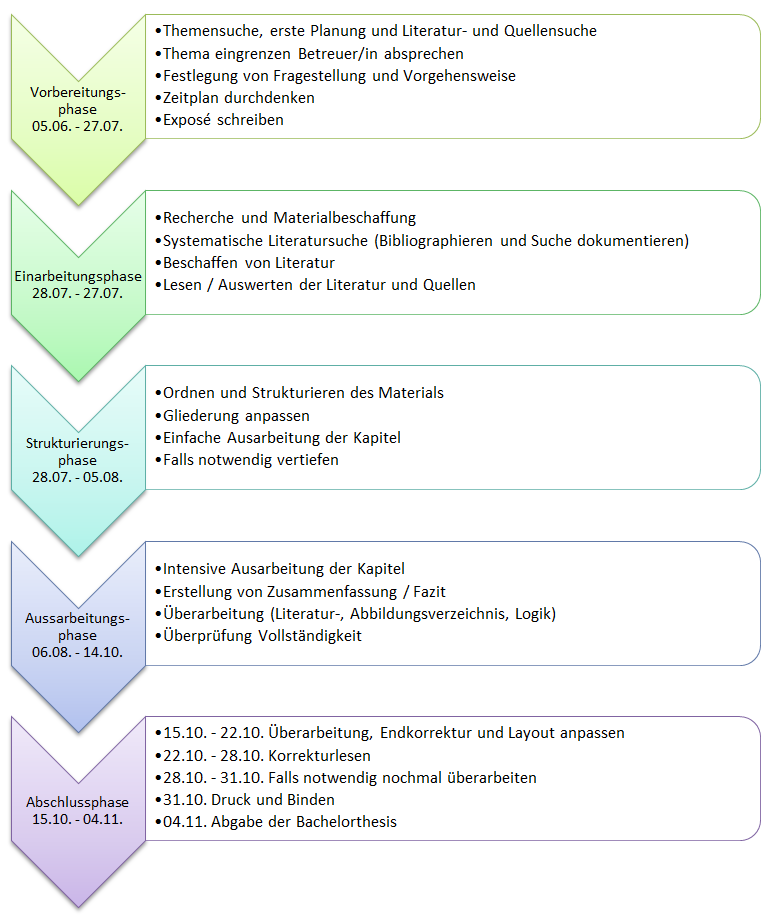
\includegraphics[scale=0.59]{images/Ablaufplan_BA.png}
 \caption{Ablaufplan der Vorgehensweise}
 \label{fig:Ablaufplan-BA}
\end{figure}

%%% Local Variables: 
%%% mode: latex
%%% TeX-master: "thesis"
%%% End: 
